\title{Home is where the help is: \\ \emph{How childcare assistance shapes Twe women's residence}}
\author{
        Layne Vashro \\
        Department of Anthropology\\
        University of Utah\\
}
\date{\today}

\documentclass[10pt]{article}
\usepackage{graphicx}
\usepackage[font={small}, justification=justified, singlelinecheck=false]{caption}
%\usepackage{wasysym}
\usepackage{float}
\usepackage[section]{placeins}
\usepackage{apacite}
\setlength{\parskip}{0.10cm plus2.5mm minus2.5mm}
\usepackage{natbib}
\RequirePackage{lineno}

\makeatletter
\newcommand\ackname{Acknowledgements}
\if@titlepage
  \newenvironment{acknowledgements}{%
      \titlepage
      \null\vfil
      \@beginparpenalty\@lowpenalty
      \begin{center}%
        \bfseries \ackname
        \@endparpenalty\@M
      \end{center}}%
     {\par\vfil\null\endtitlepage}
\fi
\makeatother

\begin{document}
\maketitle

\begin{abstract}         % submission
This paper uses access to childcare assistance to explain variability in women's residence among the Twe people living on the western border between Namibia and Angola.  I test the hypothesis that women are more likely to move away from their mothers when they either do not have infant children in need of childcare, or they have older daughters who can act as a secondary source of care in an alternative residence.  This relationship may be the key to understanding why women in foraging societies often delay dispersal until after they have weaned at least their first child.  The findings support this interpretation, showing that women with infants are more likely to live with their mothers, while women with older daughters are more likely to move away.  This relationship between residence and basic household demographics that are expected to shift throughout a woman's reproductive career help explain why Twe women move away from home as they age, and potentially why we see a similar pattern in many other populations.


\end{abstract}               %submission

\bigskip

\modulolinenumbers[5]
\linenumbers

\section{Introduction}

People in most small-scale societies must look outside of their residence group for viable marriage partners.  This practice of exogamy leads to at least one spouse moving away from his or her family following marriage.  In a world where family is the central source of economic, social, and political relationships, the decision of which spouse leaves home has powerful implications.  One such implication is that women lose access to the childcare assistance provided by their mothers.  This paper looks at marital residence decisions from the perspective of women seeking childcare assistance, and uses the incentive of extra-maternal care to help explain residence among the Twe of northwestern Namibia.

Since the inception of the field, anthropologists have been interested in understanding the variable ways in which people manage the problem of postmarital residence \citep{morgan1851league, tylor1889method}.  Most of this research uses group-level phenomena such as subsistence focus, warfare, and population crashes to explain variation in postmarital residence cross-culturally \citep{lippert1931evolution, murdock1949social, korotayev2003division, linton1964study, ember1971conditions, divale1974migration, elman1962primitive, ember1972conditions}.  However, recent analyses demonstrate considerable variability in the actual patterns of residence within populations in addition to the variability that exists cross-culturally.  This is especially true for simple hunter-gatherers and other groups with limited heritable wealth \citep{lee1972kung, devore1968man, alvarez2004residence, marlowe2004marital, hill2011co, walker2013living}.  Not only do different couples often come to different residence decisions in these societies, but each couple is likely to adopt a variety of strategies over time.  Many previous approaches to understanding residence are only applicable to differences between groups, and thus new approaches are needed to help understand the patterning of groups with ``flexible'' residence.  

There are undoubtedly many different factors that shape individual residence decisions.  This paper investigates the role of women seeking access to childcare assistance as one potentially influential factor.  Cross-culturally, the majority of extra-maternal childcare comes from a woman's close female relatives \citep{euler1996discriminative, hawkes1997hadza, ivey2000cooperative, sear2000maternal, voland2002opposite}.  This is important with respect to residence because a woman's mother and sisters are unavailable if she moves to live with her husband's family.  Cohabitating with these key relatives, especially the postfertile maternal grandmother, is associated with increased child survival and is a stated preference of many women among the Twe and other populations \citep{sear2008keeps, woodburn1968stability, meehan2005effects}.  

Blurton-Jones investigated the relationship between residence and childcare among the Hadza from the perspective of postfertile women optimizing investment in their grandchildren \citep{jones2005hadza}.   Hadza grandmothers were both more likely to live with daughters than sons and more likely to live with daughters who were nursing infants than those who were not.  Scelza finds that married women among the strictly virilocal Himba use temporary visits home to access female relatives, especially during pregnancy \citep{scelza2011female}.  This pattern shows that even in situations where women are unable to maintain regular contact with their families, access to childcare influences residence during peak periods of need.  The Twe actually neighbor the Himba and practice the same set of cultural traditions.  However, possibly due to differences in heritable wealth, Twe residence patterns are more flexible \citep{vashro2014diss}.  This paper uses that flexibility to assess whether consistent access to childcare assistance influences women's residence decisions.

The lure of potential childcare assistance creates a clear incentive for women to remain home.  However, not all close female relatives are tied to a woman's natal camp.  Even as young as 6 or 7 years old, prefertile girls begin directing childcare towards their younger siblings \citep{zeller1987role, kramer2004reconsidering, hames1988allocation, denham1974infant, dunbar2002helping}.  Behavioral observations find that a child's older sisters are responsible for more direct care than any relative-class other than the mother herself in many societies \citep{kramer2005children}.  This intrasibling care is associated with a collection of fitness-enhancing maternal effects, including decreased interbirth intervals, extended fertile period, increased rates of child survival, and increased leisure time \citep{turke1988helpers, Bereczei2002helping, crognier2001helpers, bove2002girl}.  With respect to residence, babysitting daughters are interesting because they provide a source of care that a woman can take with her when she moves.  This potentially frees women to respond to other residence incentives without sacrificing access to a secondary source of childcare.  In addition to looking at whether women stay home when they need childcare assistance, this paper also investigates the hypothesis that women are more likely to live away from home when they have daughters old enough to subsidize childcare in an alternative location.  

\section{Materials and Methods}

\subsection{Population}

The Twe are a population of approximately 3,000 people living in the dry and mountainous region surrounding the Kunene River in northwestern Namibia and southwestern Angola.  Their material and ritual culture mirrors that of the well-studied Himba, but they are locally viewed as an outsider ethnic group \citep{estermann1976ethnography, malan1974herero, bollig2006risk}.  The Twe practice a mixed subsistence that includes gardening, hunting and gathering, animal husbandry, and the sale of crafted and foraged goods \citep{bollig2004hunters}.  Men and women appear to contribute relatively equally to subsistence, and neither sex controls considerable heritable wealth.

The typical Twe household includes the nuclear family and some extended kin.  Households often shift location between a rainy season camp near the family's garden and dry season camps in or near the mountains.  Especially during the wet season, households cluster into villages along seasonal rivers, with households spaced within several kilometers of one another.  Village populations typically range from 10 to 30 adults, while one recently established government camp with a school, clinic, and water-tower has 40 adults living nearby.  This study includes 40 different households spread across 19 villages and looks at women's movement between these residences throughout their reproductive careers.  

Most Twe women start their reproductive careers between ages 19 and 22.  The average interbirth interval of Twe women is 3.4 years and approximately 12\% of children die during infancy (this estimate comes from interviews which likely under-report actual rates of infant mortality).  The average Twe woman has 4.2 living children when she finishes her reproductive career (estimated by averaging across all women between ages 45 and 55).

Men occasionally promise their daughters to other men, but these marriages are not made official until the girl reaches menarche and rarely come to fruition due to the young woman's objections.  A man may also arrange to marry an adult woman through her father.  These marriages account for about 43\% of marriages, while the rest involve a man first successfully courting a woman then going to her father to ask permission.  Only 15\% of married men have more than one wife.  These polgynous marriages have minimal direct impact on young women, since none of the cowives in my data are under the age of 30 and their mean age is 50 years old.   

The Twe do not recognize any formal system of bride service.  Bride wealth is culturally expected, but rarely exceeds small gifts like sacks of maize meal, blankets, and buckets of honey.  Most Twe participants say that a woman is supposed to move away from her family and live with her husband and his family following marriage.  This is consistent with the Himba rule of virilocal residence. However, observed patterns of residence are not consistent with this rule.  Most couples actually stay with the wife's family early in the relationship, and less than 40\% of husbands ever bring their wives to live in their familial village.  

\subsection{Procedure}

\subsubsection{Observational scans} 
Children's maternal grandmothers and older sisters are reliable sources of childcare assistance in many populations.  However, there remains considerable cross-cultural variability in the child-caring role of different relative classes \citep{hames2004women, kramer2010cooperative}.  I used observational scans to assess the childcare role of different relatives among the Twe \citep{crittenden2008allomaternal}.  These scans took place in a single village between December 2010 and February 2011.  This particular village was chosen because it offered the largest aggregation of Twe people, with 20 to 30 individuals within easy walking distance at a given time.  This allowed both the collection of a larger sample in shorter time as well as a greater variety of possible childcare interactions because a broader range of relatives were available.

Initial scans were made each hour between 7 in the morning and 7 in the evening by walking an approximately 1 kilometer circuit through the village and recording all instances of someone holding a child under the age of 3, then reversing the route taken on the next scan.  Participants began tending their gardens in late January.  This stretched the camp boundaries and increased the route to more than 2 kilometers, which was too large an area to reasonably cover on an hourly basis.  Camp scans during these final 2 weeks were conducted every 2 hours.

\subsubsection{Residence history interviews}  
In order to assess the relationship between access to childcare and women's residence decisions, I used interviews to identify current and historical residence locations of women and their relatives.  I interviewed 176 participants about contemporary residence in years 2010 and 2012 and historical residence during 1990, 2001, and 2006.  The 3 earlier years were chosen because each had some salient event that made it easier to accurately recall.  I also collected historical residence data from 1974 and 1983, but do not include those years in these analyses because reports were less reliable between participants and the precision of children's age estimates become considerably noisier that far back in time.  I asked participants where they lived in each year, and then using previously collected genealogies asked where each of their parents, siblings, children, grandparents, spouses, spouses' primary relatives, aunts, and uncles lived during that time.  Many Twe stay in multiple different locations within a given year but recognize a single location as their ``home,'' which is what I use in these analyses.  Seasonal residence shifts are typically made as a household unit, meaning that the available relatives remain static even if actual location changes.  That said, individuals do travel away from the household within a given year for a variety of reasons, which makes the actual access to kin more complex than what is captured in these data.

\subsection{Analyses}
The data were analyzed using logistic regression models and data visualization techniques to test assumptions of normality.  I conducted all data analysis using R 2.15.1 statistical software \citep{rdevcore}.

\section{Results}

\subsection{Do Twe grandmothers and sisters provide childcare?}  
Mothers, older sisters, maternal aunts, maternal grandmothers, and female cousins in the maternal line were the relative classes most often observed holding young children.  After adjusting for the number of individuals in each relative class in camp during an instance of holding, mothers, older sisters, and the maternal grandmother stand out as the most active carers (see Table \ref{tab:whocares}).  After mothers, older sisters have the highest ``holding ratio'' of all relative classes, being the individual holding a young child in 15 cases out of 80 opportunities.  There were 51 cases of a maternal grandmother being available during a holding event and in 7 of those cases, she was the one holding the child.  The next highest ratio was maternal female cousins who held a young child in 9\% of opportunities.  The sample size for these observations is quite small (28 days and 407 caring events) and limited to a single camp, but they support the assumption that the mother, maternal grandmother, and older sisters are the key sources of direct childcare among the Twe.  This pattern is also consistent with women's self-reports of who they can expect to help take care of their children. 

\begin{table}[!tb]
\caption {Who cares? \label{tab:whocares} }
  \centering
  \begin{tabular}{| l | l | l | l |} 
  	\hline
	\emph{Relationship} & \emph{Holder} & \emph{Available} & \emph{Percentage}\\ \hline
	Mother & 292 & 398 & 73\%\\	
	Older sister & 15 & 80 & 18.8\%\\	
	Mat. Grandmother & 7 & 51 & 13.7\%\\	
	Mat. Cousin (f) & 8 & 90 & 8.9\%\\
	Father & 8 & 124 & 6.5\%\\
	Pat. Aunt & 1 & 16 & 6.2\%\\
	Mat. Aunt & 10 & 320 & 3.1\%\\ \hline
  \end{tabular}    
  
{Includes all relative classes observed holding a young child in at least 1\% of opportunities. `Mat.' and `Pat.' are used to discriminate between maternal and paternal relatives.}
\end{table}

\subsection{Does women's residence map onto childcare assistance?}  
Analyses use logistic regression with the dependent variable set as whether or not a woman lives with her mother.  The dataset includes 86 unique women under the age of 45 with at least one child and a living mother.  These women account for 198 observations across the 4 years of residence data.  Because the data-set includes multiple observations of the same women, it is important to account for potential data dependency issues.  Each woman likely possesses different underlying characteristics that relate to childcare and residence in ways that are not captured in the data.  In order to address this issue, I use linear mixed-effect models (LMEMs, function lme4 package \citep{bates2011lmer}) that include by-participant random effects.  Each LMEM includes by-participant random intercepts and random slopes for all critical variables when possible.  This approach of using the maximal random effect structure minimizes Type \textrm{I} error \citep{barr2013random, schielzeth2009conclusions}.  However, the median participant was only observed twice.  This constrains model complexity and forces the omission of some random slopes which ideally should be included in the models. 

\begin{table}[!tb]
\caption {When do women live with their mothers? \label{tab:bbsit} }
  \centering
  \begin{tabular}{| l | r r | r r | r r | r r |} 
  	\hline
	\emph{IV} & \multicolumn{2}{|c|}{\emph{Model 1}} & \multicolumn{2}{|c|}{\emph{Model 2}} & \multicolumn{2}{|c|}{\emph{Model 3}} & \multicolumn{2}{|c|}{\emph{Model 4}}\\ 
	& \emph{B} & \emph{SE B} & \emph{B} & \emph{SE B} & \emph{B} & \emph{SE B} & \emph{B} & \emph{SE B}\\ \hline
	Young children & \textbf{1.03} & \textbf{0.32} & \textbf{1.06} & \textbf{0.37} & \textbf{0.88} & \textbf{0.38} & \textbf{1.29} & \textbf{0.46} \\	
	Babysitters &  &  & \textbf{-1.75} & \textbf{0.48} & \textbf{-1.58} & \textbf{0.50} & \textbf{-1.58} & \textbf{0.54} \\
	Age & & & & & -0.04 & 0.04 & 0.00 & 0.05 \\
	Married? & & & & & & & \textbf{-3.52} & \textbf{0.66} \\
	AIC & \multicolumn{2}{|c|}{\textbf{246.1}} & \multicolumn{2}{|c|}{\textbf{238.2}} & \multicolumn{2}{|c|}{239.4} & \multicolumn{2}{|c|}{\textbf{208.6}}\\ 
	ICC & \multicolumn{2}{|c|}{.55} & \multicolumn{2}{|c|}{.54} & \multicolumn{2}{|c|}{.42} & \multicolumn{2}{|c|}{.75}\\ \hline
  \end{tabular}  
{Unstandardized betas and standard error of each coefficient in models 1, 2, 3, and 4.  Bold values indicate statistical significance ($p < .05$).  ICC calculation follows \citep{zeger1988models}.}
\end{table}

Model 1 investigates whether women are more likely to live with their mother when they have young children.  The model includes the number of children younger than 3 a woman has as a lone independent variable.  Model 1 and all subsequent models omit by-participant random slopes for the ``young children'' variable because its inclusion makes the model too complex given the limited observations for each participant.  This problem is seen in a weakened AIC score and deterministic negative correlation between the random slope and intercept.  The fixed-effect for the ``young children'' variable is a significant predictor of women's coresidence with their mothers (see Table \ref{tab:bbsit}).  Seventy-one percent of women with at least one young child live with their mother, while only 55\% of women without a young child live with their mother.

The second model retains the ``young children'' variable but also looks at whether daughters old enough to take on a babysitting role, but still too young to have started their own reproductive career (age 6 to 15), allow women to move away from home.  This model also includes a by-participant random slope effect for the `babysitters' variable.  Model 2 is a significant improvement over Model 1 (see Table \ref{tab:bbsit}).  Both the ``young children'' and ``babysitters'' fixed-effects are significant predictors of women's coresidence with their mothers, but in opposite directions.  There is also a by-participant random slope effect within the ``babysitters'' variable (variance = 4.67, \emph{SD} = 2.16, Int. Corr = -0.34).  

The next two models introduce important control variables.  When the focal woman's age is entered as a lone independent variable, it is a significant negative predictor of women's coresidence with their mothers (\emph{B} = -0.10, \emph{SE B} = 0.03, p $<$ .001).  This makes age an important confound to control for because older women are more likely to both live away from home and have older daughters.  However, the addition of age to Model 2 weakens overall performance and introduction of the age variable does not qualitatively change the relationship between young children, babysitters, and residence (see Table \ref{tab:bbsit}).  Model 3 also finds a by-participant random slope effect for the ``babysitters'' variable (variance = 4.35, \emph{SD} = 2.09, Int. Corr = -0.27).  

\begin{figure}[!tb]
    \centering
    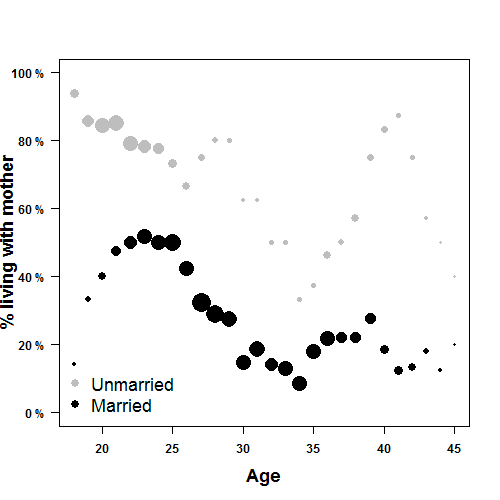
\includegraphics[scale=.7]{images/obs_crmom}
\caption{Observed rates of residence with mother \label{fig:obs_crmom} }
\medskip
The above plot gives the observed rate of women's coresidence with their mothers at each age $+$ or $-$ 2 years.  The size of points indicates the relative size of sample at each age.
\end{figure}  

\begin{figure}[!tb]
    \centering
    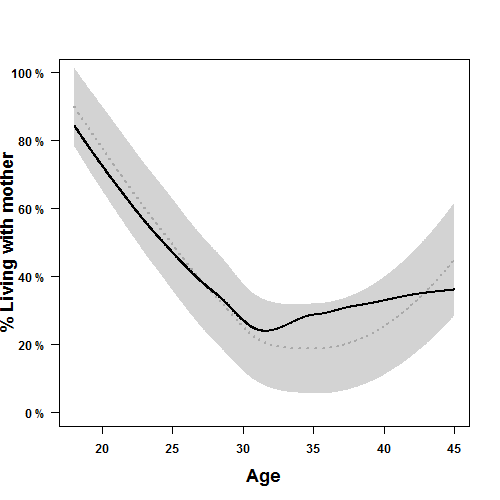
\includegraphics[scale=.55]{images/babysit}
\caption{Predicted probability of living with mother across ages \label{fig:bbsit_fig} }
\medskip
The solid black line gives the observed percent of Twe women living with their mothers at each age from 18 to 45.  The dotted gray line is the predicted probability that a woman lives with her mother at each age using Model 3 (see Table \ref{tab:bbsit}) and the age-specific means of young children, babysitters, and being married.  The light gray shaded area gives that confidence interval around that predicted probability.
\end{figure}

Model 4 adds the focal woman's marital status as an additional control.  Marriage is an important control because 40\% of women in the sample are not married and there is a clear relationship between marriage and women's coresidence with their mothers.  Seventy-three percent of unmarried women live with their mother compared to 28\% of married women (see Figure \ref{fig:obs_crmom}).  The addition of the marriage variable significantly improves model performance but does not qualitatively change the influence of young children and babysitters  (see Table \ref{tab:bbsit}).  Model 4 also continues to find a by-participant random slope effect within the ``babysitters'' variable (variance = 3.96, \emph{SD} = 2, Int. Corr = -0.45).  Finally, after including marital status, the relationship between age and women's residence with their mothers has been completely explained by the other variables in the model (see Figure \ref{fig:bbsit_fig}).  

One possible explanation for why offspring composition continues to explain residence beyond the powerful effect of marriage is that young women without babysitting daughters are less likely to be married (see Model 5 in Table \ref{tab:mar_bbsit_tab} and Figure \ref{fig:mar_bbsit}).  This relationship is not simply a function of married women having more children, as the effect remains even after controlling for the total number of children a woman has (see Model 6 in Table \ref{tab:mar_bbsit_tab}).  Models 5 and 6 also included only by-participant random slopes for the ``babysitters'' variable because more complex models failed to converge (Model 5: variance = 4.05, \emph{SD} = 2.01, Int. Corr = -0.93; Model 6: variance = 4.07, \emph{SD} = 2.02, Int. Corr = -0.91). 

\begin{table}[!tb]
\caption {Babysitters and marriage \label{tab:mar_bbsit_tab} }
  \centering
  \begin{tabular}{| l | r r | r r |} 
  	\hline
	\emph{IV} & \multicolumn{2}{|c|}{\emph{Model 5}} & \multicolumn{2}{|c|}{\emph{Model 6}}\\ 
	& \emph{B} & \emph{SE B} & \emph{B} & \emph{SE B} \\ \hline
	Babysitters & \textbf{4.82} & \textbf{2.40} & \textbf{4.81} & \textbf{2.45} \\	
	Age  & \textbf{0.17} & \textbf{0.05} & \textbf{0.15} & \textbf{0.06} \\
	Babysitters X Age & \textbf{-0.15} & \textbf{0.07} & \textbf{-0.15} & \textbf{0.07} \\
	Total children & & & 0.09 & 0.17 \\
	AIC & \multicolumn{2}{|c|}{\textbf{261.9}} & \multicolumn{2}{|c|}{263.6}\\
	ICC & \multicolumn{2}{|c|}{.89} & \multicolumn{2}{|c|}{.89}\\ \hline
  \end{tabular}  
  
{Unstandardized betas and standard error of each coefficient in models 5 and 6.  Bold values indicate statistical significance ($p < .05$).  ICC calculation follows \citep{zeger1988models}.}
\end{table}

\begin{figure}[!tb]
    \centering
    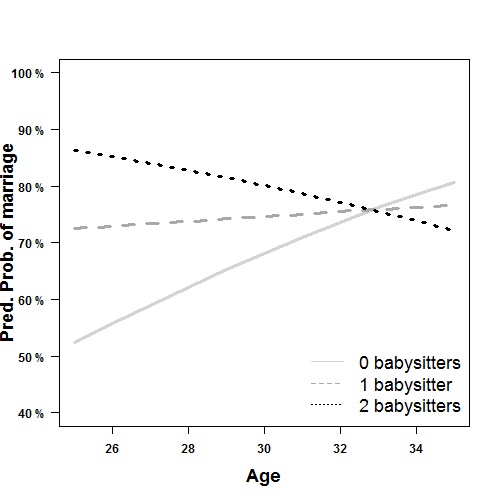
\includegraphics[scale=.55]{images/mar_bbsit}
\caption{Predicted probability of living with mother \label{fig:mar_bbsit} }
\medskip
Model 5 predicted probability plot for ages 25 to 35 for women with 0, 1, or 2 babysitters.
\end{figure}

In order to test whether the babysitter effect actually captures something unique to girls in that age-group, I replaced the babysitter variable in models 2, 3, and 4 with one representing the number of boys a woman has in that same 7 to 15 years old age range.  The number of older boys a woman has is only a significant predictor in the modified Model 2, and this effect is diminished after reintroducing the babysitter variable (\emph{B} = -0.27, \emph{SE B} = 0.23, p = .23) showing that the impact of older boys is likely a function of their covariance with older girls. 

Since the negative relationship between having a babysitter and women living near their mothers is assumed to be a function of decreased dependency on childcare assistance coming from the maternal grandmother, we should expect the effect to be less pronounced when women do not have young children.  The final model adds an interaction effect between the young children and babysitters variables along with marital status as a control.  The interaction term in this model is in the expected direction but is not a significant predictor of women's residence (\emph{B} = -0.92, \emph{SE B} = 1.20, \emph{p} = .44).               

\section{Discussion and Conclusions}

Maternal grandmothers and older sisters are the most reliable sources of extra-maternal childcare among the Twe.  This is consistent with other empirical work investigating childcare in traditional societies.  Twe women are more likely to live with their mother when they have more young children and thus greater demand for childcare assistance.  In addition, Twe women take advantage of the residence flexibility offered by babysitting daughters who are tied to them rather than any particular camp.  The findings in this paper demonstrate that childcare assistance is a residence incentive that women will map onto when not overwhelmed by other factors.  This understanding is an important step towards describing residence variability.  In particular, the opposing residence effects of young children and older daughters may help explain one commonly observed pattern in societies practicing ``flexible'' residence.  

Women often remain with their families early in their reproductive career but then later move away.  This pattern is seen across a wide variety of societies, but is particularly common among foragers and other groups with limited access to material wealth \citep{marshall1959marriage, marlowe2004marital, hill2011co_sup}.  Participant reports often associate this pattern with young mothers needing the childcare assistance of their family \citep{lee1982politics}, but the logic of this explanation is not immediately intuitive.  Young mothers may benefit more from the childcare assistance available in their natal residence due to the costs associated with maternal inexperience \citep{hrdy2007evolutionary}.  However, women's demand for assistance is likely to increase rather than decrease as they progress through their reproductive careers and accrue children.  The key to solving this riddle may lie in looking not just at changes in the need for care but also changes in the source of care and how different sources create different residence incentives.  I show in the previous chapter that we can expect care from older sisters to replace care from the maternal grandmother and aunts as a woman progresses through her reproductive career, thus shifting the dependence on assistance from relatives tied to the maternal camp to a portable source of care.  This paper's findings are consistent with that explanation.

The Twe add an interesting wrinkle to this pattern in that the majority of married women move away from their family even when they are young.  However, Twe women often delay marriage until they have a daughter old enough to act as a secondary childcare provider in their husband's household.  The Twe have an unusually high rate of unmarried mothers and the trade-off between marriage and living near family may explain why.  Strict adherence to a rule of virilocal residence makes sense in a population like the Himba where men control considerable resources and thus hold a dominant bargaining position.  When there is a mismatch between the cultural expectations of marriage and the benefits that marriage offers, it may be advantageous for a woman to take lovers or have a stable but unofficial partner while remaining in her natal household until she is in a better position to move away from her mother.

Cooperative childcare is an influential factor shaping household composition, at least among the Twe and the Hadza \citep{jones2005hadza}.  However, not all women have the option of turning to their mother for assistance.  This study only looked at women with living mothers, but 26\% of Twe infants are born without a living maternal grandmother.  Other factors including the presence of prefertile aunts, competition between cousins for the maternal grandmother's care, and the relative interest of the paternal grandmother were not addressed in this paper but should add to the variability of individual residence decisions based on childcare assistance.  The relative availability of childcare assistance in the natal camp differs across women for many reasons and this is consistent with the by-participant random effects found in this study.  These differences may offer an important tool for understanding not just the specific pattern of women moving away from home as they progress in their reproductive career, but also the highly variable residence patterns of women and married couples within the majority of foraging societies.

\section*{Acknowledgements}
We are grateful to the Twe people for their participation and hospitality.  We also thank Steven Josephson and Polly Wiessner for their assistance in establishing a fieldsite in the Kunene Region. Data collection by the first author was supported by both NSF grant 1026373 and the Wenner-Gren Foundation.

\section*{Data accessibility}
Data used in these analyses are available from Vashro by request.

\bibliography{MyThesisRefs}
\bibliographystyle{apacite}

\end{document}

